\documentclass[a4paper]{article}

\usepackage{graphicx}
\usepackage{subcaption}
\usepackage{url}
\usepackage[T1]{fontenc}
\usepackage[utf8]{inputenc}

\begin{document}

\title{Dissem.in: Metadata Harvesting for Open Access Policies}
\author{Antonin Delpeuch \\
University of Cambridge \\
École Normale Supérieure \\
\texttt{antonin@delpeuch.eu}}

\maketitle

Many universities adopt open access policies requiring researchers to make their articles freely
available in a repository. Enforcing these policies is far from straightforward however: according to
a recent study in the UK~\cite{research2014counting},
each article costs an estimated 33 GBP of staff time to ensure policy
compliance.
Researchers often consider these policies as a burden: they need to
understand the requirements of their publishers and their institutions,
and to spend time uploading their articles to various repositories, with
the appropriate metadata.

To solve these problems, we build \emph{dissem.in}, a
system that leverages various metadata sources to get the publications
list of researchers affiliated to a given university. The tool helps
researchers to upload their papers and universities to measure the
availability of their research output in open repositories. The key
feature is that the system is not a repository itself and is not tied to
any particular repository, but is more a form of search engine.

\section{Overview of the system}

Our web platform allows to browse the publications of researchers within
a university. These publications can be filtered using two criteria:
publisher policy and full text availability.

\begin{figure}[htbp]
\centering
\begin{subfigure}[b]{0.45\textwidth}
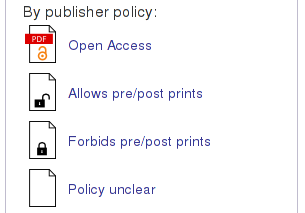
\includegraphics[scale=0.5]{img/policy.png}
\end{subfigure}
\begin{subfigure}[b]{0.45\textwidth}
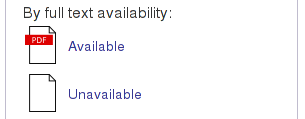
\includegraphics[scale=0.5]{img/availability.png}
\vspace{0.4cm}
\end{subfigure}
\end{figure}

These two criteria can be visually combined to help researchers grasp
instantly the status of their publications, as in the following example:

\begin{figure}[htbp]
\centering
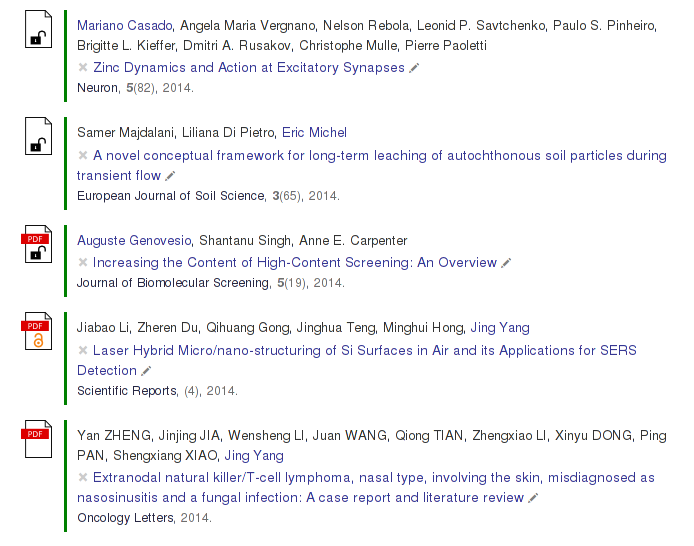
\includegraphics[scale=0.5]{img/publist.png}
\end{figure}

%The two first papers were not found in any repository, but their
%publisher's policy indicates that they could be made available. They
%would then be marked as the third paper. The fourth paper is published
%in an open access journal and is hence considered available. The last
%paper is also available and the publisher policy is marked as unknown.

\section{Demo}

A prototype is running and encompasses some departments of the École
Normale Supérieure (ENS), a french university where an open access policy
is being elaborated. It is online here:
\url{http://ens.dissem.in/}

\section{Technical details}

\subsection{Metadata sources}

We use the OAI-PMH \cite{oaipmh} protocol to crawl repositories, covering more
than 8 millions of papers. An additional coverage is provided by the Bielefeld
Academic Search Engine \cite{lossau2006bielefeld} and CrossRef.org.

\subsection{Author disambiguation}

We perform automatic author name disambiguation to get accurate
publications list for each researcher. The problem can be formulated as
follows: given a list of researchers for each department in a
university, and given a list of millions of papers fetched from various
sources, find the papers corresponding to our known researchers. Our
approach is a two-stage machine learning algorithm, similar to the AuthorMagic heuristics
used in the Invenio platform \cite{weiler2011authormagic}.

\bibliographystyle{plain}
\bibliography{references}

\end{document}

